\section{Experimental Results}
\subsection{Raw Data vs Scaled Data}
\begin{figure}[ht!]
    \centering
    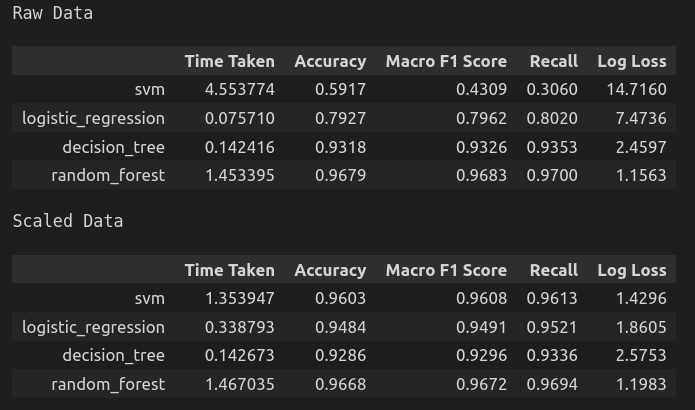
\includegraphics[width = 0.45\textwidth]{./images/raw_vs_scaled.png}
    \caption{Metrics for Raw and Scaled Data}
    \label{fig:3}
\end{figure}
The results demonstrate that data scaling significantly enhances the performance of SVM and Logistic Regression models, but has a negligible impact on Decision Tree and Random Forest models.
\subsection{Cross Validation}
\begin{figure}[ht!]
    \centering
    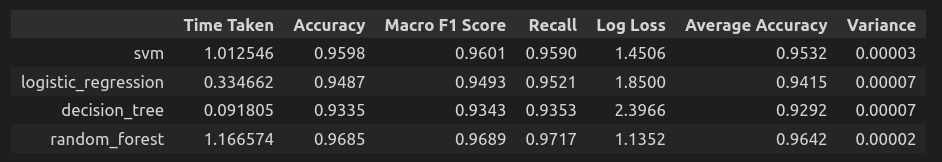
\includegraphics[width = 0.45\textwidth]{./images/k_fold.png}
    \caption{Performance Metrics}
    \label{fig:4}
\end{figure}
We used a 10-fold cross-validation for model evaluation. The first five metrics in the table represent the performance of the model, selected for its highest cross-validation accuracy, against the held-out test data (unseen data). The final two metrics reflect the model's overall performance on the entire training dataset.\\
Based on Average Accuracy, the performance hierarchy is:\\
Random Forest $>$ Support Vector Machine $>$ Logistic Regression $>$ Decision Tree.\\
The models, ranked by variance (overfitting susceptibility): \\
Decision Tree $>$ Logistic Regression $>$ Support Vector Machine $>$ Random Forest.
\subsection{Hyperparameter Tuning}
The best hyperparameters found via GridSearchCV are:\\\\
\begin{tabular}{ll}
\textbf{SVM:} & \textbf{Logistic Regression:} \\
\quad  C: 10 & \quad  C: 100.0 \\
\quad  gamma: scale & \quad penalty: l2 \\
\quad  kernel: rbf & \\
& \\
\textbf{Decision Tree:} & \textbf{ Random Forest:} \\
\quad  max\_depth: 25 & \quad  max\_depth: 25 \\
\quad  min\_samples\_leaf: 5 & \quad  max\_leaf\_nodes: 450 \\
\quad  min\_samples\_split: 30 & \quad  min\_samples\_split: 1 \\
\end{tabular}
\begin{figure}[ht!]
    \centering
    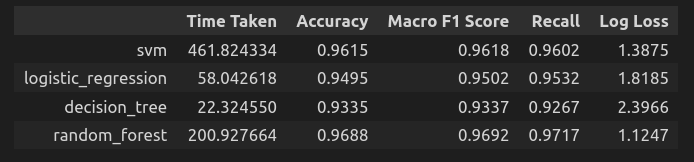
\includegraphics[width = 0.45\textwidth]{./images/gridsearchcv.png}
    \caption{Metrics of the refitted/tuned models}
    \label{fig:5}
\end{figure}\\
The \textit{Time Taken} values indicate the time required to train all grid-searched hyperparameter combinations with cross-validation.
\subsection{Majority Voting}
\begin{figure}[ht!]
    \centering
    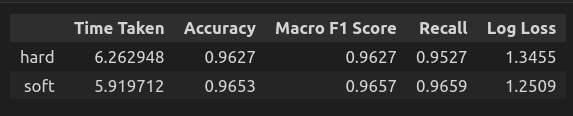
\includegraphics[width = 0.45\textwidth]{./images/majority.png}
    \caption{Hard and Soft Majority Voting}
    \label{fig:6}
\end{figure}
As expected, soft majority voting's accuracy is higher than hard voting's, as shown in the table.
\begin{figure}[ht!]
    \centering
    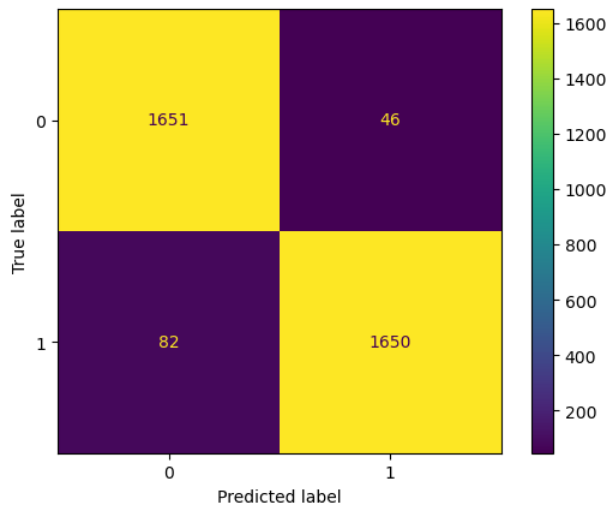
\includegraphics[width = 0.45\textwidth]{./images/conf_hard.png}
    \caption{Confusion Matrix of Hard Majority}
    \label{fig:7}
\end{figure}
\begin{figure}[ht!]
    \centering
    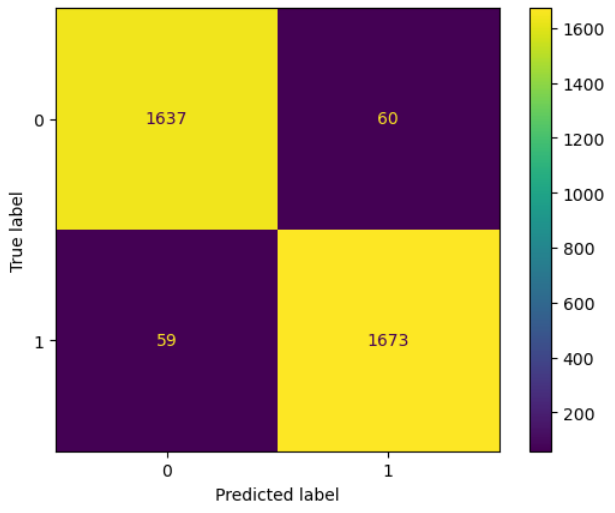
\includegraphics[width = 0.45\textwidth]{./images/conf_soft.png}
    \caption{Confusion Matrix of Soft Majority}
    \label{fig:8}
\end{figure}
\begin{figure}[ht!]
    \centering
    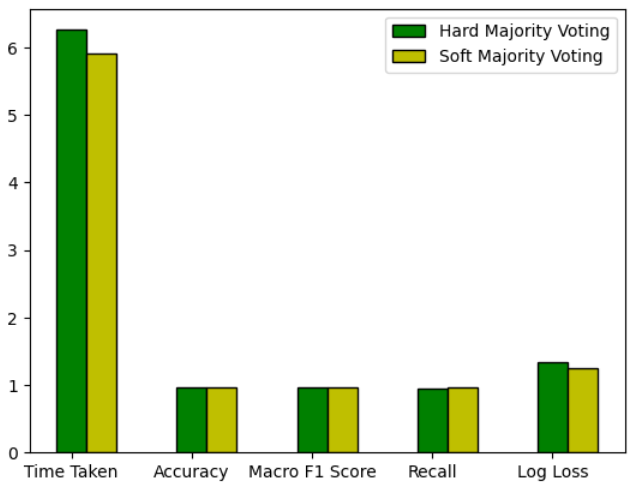
\includegraphics[width = 0.45\textwidth]{./images/hard_soft.png}
    \caption{Hard vs Soft Majority}
    \label{fig:9}
\end{figure}
\section{Discussion}
\begin{itemize}
    \item Random Forest exhibits the highest average accuracy and lowest variance, but requires increased training time.
    \item Support Vector Machine demonstrates performance comparable to Random Forest, with slightly lower accuracy but a slightly higher training time, and variance.
    \item Logistic Regression offers moderate performance with average training time.
    \item Decision Tree achieves the fastest training time, but suffers from the lowest accuracy and highest variance.
\end{itemize}
\section{Improvements}
\begin{itemize}
    \item[-] Further performance improvements could be explored by evaluating feature combinations, in addition to individual features.
    \item[-] Feature selection techniques, such as chi-square or Pearson correlation, could be employed to identify and utilize the most relevant features, potentially enhancing model performance.
    \item[-] Real-time classification could be implemented, similar to a website extension. However, this would necessitate optimizing feature extraction for reduced runtime.
\end{itemize}